\documentclass{article}

\usepackage[T1]{fontenc}

\usepackage{fancyhdr} % Required for custom headers
\usepackage{lastpage} % Required to determine the last page for the footer
\usepackage{extramarks} % Required for headers and footers
\usepackage[usenames,dvipsnames]{color} % Required for custom colors
\usepackage{graphicx} % Required to insert images
\usepackage{listings} % Required for insertion of code
\usepackage{courier} % Required for the courier font
\usepackage{lipsum} % Used for inserting dummy 'Lorem ipsum' text into the template
\usepackage{hyperref}

% Margins
\topmargin=-0.45in
\evensidemargin=0in
\oddsidemargin=0in
\textwidth=6.5in
\textheight=9.0in
\headsep=0.25in

\linespread{1.1} % Line spacing

% Set up the header and footer
\pagestyle{fancy}
\lhead{\hmwkAuthorName} % Top left header
\chead{\hmwkClass\ (\hmwkClassInstructor\ \hmwkClassTime): \hmwkTitle} % Top center head
\rhead{\firstxmark} % Top right header
\lfoot{\lastxmark} % Bottom left footer
\cfoot{} % Bottom center footer
\rfoot{Page\ \thepage\ of\ \protect\pageref{LastPage}} % Bottom right footer
\renewcommand\headrulewidth{0.4pt} % Size of the header rule
\renewcommand\footrulewidth{0.4pt} % Size of the footer rule

\setlength\parindent{0pt} % Removes all indentation from paragraphs

\usepackage{listings}
\usepackage{color}
\usepackage{hyperref}

\definecolor{dkgreen}{rgb}{0,0.6,0}
\definecolor{gray}{rgb}{0.5,0.5,0.5}
\definecolor{mauve}{rgb}{0.58,0,0.82}

\lstset{frame=tb,
  language=Java,
  aboveskip=3mm,
  belowskip=3mm,
  showstringspaces=false,
  columns=flexible,
  basicstyle={\small\ttfamily},
  numbers=none,
  numberstyle=\tiny\color{gray},
  keywordstyle=\color{blue},
  commentstyle=\color{dkgreen},
  stringstyle=\color{mauve},
  breaklines=true,
  breakatwhitespace=true
  tabsize=3
}

%----------------------------------------------------------------------------------------
%	DOCUMENT STRUCTURE COMMANDS
%	Skip this unless you know what you're doing
%----------------------------------------------------------------------------------------

% Header and footer for when a page split occurs within a problem environment
\newcommand{\enterProblemHeader}[1]{
\nobreak\extramarks{#1}{#1 continued on next page\ldots}\nobreak
\nobreak\extramarks{#1 (continued)}{#1 continued on next page\ldots}\nobreak
}

% Header and footer for when a page split occurs between problem environments
\newcommand{\exitProblemHeader}[1]{
\nobreak\extramarks{#1 (continued)}{#1 continued on next page\ldots}\nobreak
\nobreak\extramarks{#1}{}\nobreak
}




%----------------------------------------------------------------------------------------
%	NAME AND CLASS SECTION
%----------------------------------------------------------------------------------------

\newcommand{\hmwkTitle}{Git guide} % Assignment title
\newcommand{\hmwkDueDate}{Martedi,\ Aprile 15,\ 2015} % Due date
\newcommand{\hmwkClass}{Ingegneria del Software 1} % Course/class
\newcommand{\hmwkClassTime}{} % Class/lecture time
\newcommand{\hmwkClassInstructor}{Carlo Ghezzi} % Teacher/lecturer
\newcommand{\hmwkAuthorName}{} % Your name

%----------------------------------------------------------------------------------------
%	TITLE PAGE
%----------------------------------------------------------------------------------------

\title{
\vspace{2in}
\textmd{\textbf{\hmwkClass:\ \hmwkTitle}}\\
\normalsize\vspace{0.1in}\small{Due\ on\ \hmwkDueDate}\\
\vspace{0.1in}\large{\textit{\hmwkClassInstructor\ \hmwkClassTime}}
\vspace{3in}
}

\author{\textbf{\hmwkAuthorName}}
\date{} % Insert date here if you want it to appear below your name

%----------------------------------------------------------------------------------------

\begin{document}

\maketitle

%----------------------------------------------------------------------------------------
%	TABLE OF CONTENTS
%----------------------------------------------------------------------------------------

%\setcounter{tocdepth}{1} % Uncomment this line if you don't want subsections listed in the ToC

\newpage
\tableofcontents
\newpage



%----------------------------------------------------------------------------------------

 \section{Preliminaries}

A version control system is a piece of software that helps the
developers on a software team work together and also archives a
complete history of their work.

There are three basic goals of a version control system (VCS):

\begin{enumerate}
\item We want people to be able to work simultaneously, not serially.
\item When people are working at the same time, we want their changes
  to not conflict with each other
\item We want the keep the complete evolution of the code
\end{enumerate}

\subsection*{History}
Broadly speaking, the history of version control tools can be divided
into three generations.

\subsubsection*{The first generation - Local revision systems}

The common trait of first generation of VCSes was that they were all
file-oriented and centralized. Most were locking-based, with
merging-based systems arriving towards the end of that era. Only one
person could be working on a file at a time. 

\subsubsection*{The second generation - Centralized revision systems}

The second generation tools are a fair bit more permissive about
simultaneous modifications, with one notable restriction. Users must
merge the current revisions into their work before they are allowed to
commit. 

Example: Subversion (SVN)

It is clearly the best of the centralized VCSes, but just as clearly
the last of its kind. As dispersed, Internet-mediated software
development becomes the norm rather than the exception, the
centralized model of version control is visibly running out of steam.

\subsubsection*{The third generation - Distributed revision systems}

Third-generation VCSes are natively decentralized. Each user maintains
his own local repository and changes from multiple users are merged 
into the remote repository.

Example: BitKeeper (BK)

BitKeeper is a merging, changeset-oriented, decentralized,
commit-before-merge VCS designed by Larry McVoy.
He decided to use Linux kernel as a reference project and he designed
the system to support the heavily decentralized and patch-oriented
style of the Linux kernel developers.

In 2002 McVoy successfully persuaded Linus Torvalds to adopt BitKeeper
and its proprietary software license. On 1 July 2005,
McVoy withdrew the free version that kernel developers had
been using and Torvalds promptly abandoned BitKeeper and moved
to design an open-source version. This meant that several BitKeeper
ideas became central in later VCS designs, notably the
representation of history as a changeset-based DAG,
commit-before-merge operation, and the semantics of the associated
push and pull operations.

Finally, two others VCS (Mercurial and git) were launched with
the same objective by Linux kernel developers who had had extensive
experience with BitKeeper.\footnote{For more on history of git watch
  Linus' talk at Goole \url{https://www.youtube.com/watch?v=4XpnKHJAok8}}



% \subsection{Features}

\section{Usage}

\subsection{Setting up the repository}

\subsubsection*{git init}

The git init command creates a new Git repository. It can be used to
convert an existing, unversioned project to a Git repository or
initialize a new empty repository. Most of the other Git commands are
not available outside of an initialized repository, so this is usually
the first command you'll run in a new project. 

Executing git init creates a .git subdirectory in the project root,
which contains all of the necessary metadata for the repo. Aside from
the .git directory, an existing project remains unaltered (unlike SVN,
Git doesn't require a .git folder in every subdirectory). 

\begin{lstlisting}
$ git init
\end{lstlisting}

Create an empty Git repository in the specified directory. Running
this command will create a new folder called <directory> containing
nothing but the .git subdirectory.

\begin{lstlisting}
$ git init --bare <directory>
\end{lstlisting}

Shared remote repositories should always be created with the --bare
flag. In fact, the remote repositiory that you are going to be using in the
class is already going to be initialized, however you are responsible
for creating your local repositories.

\begin{center}
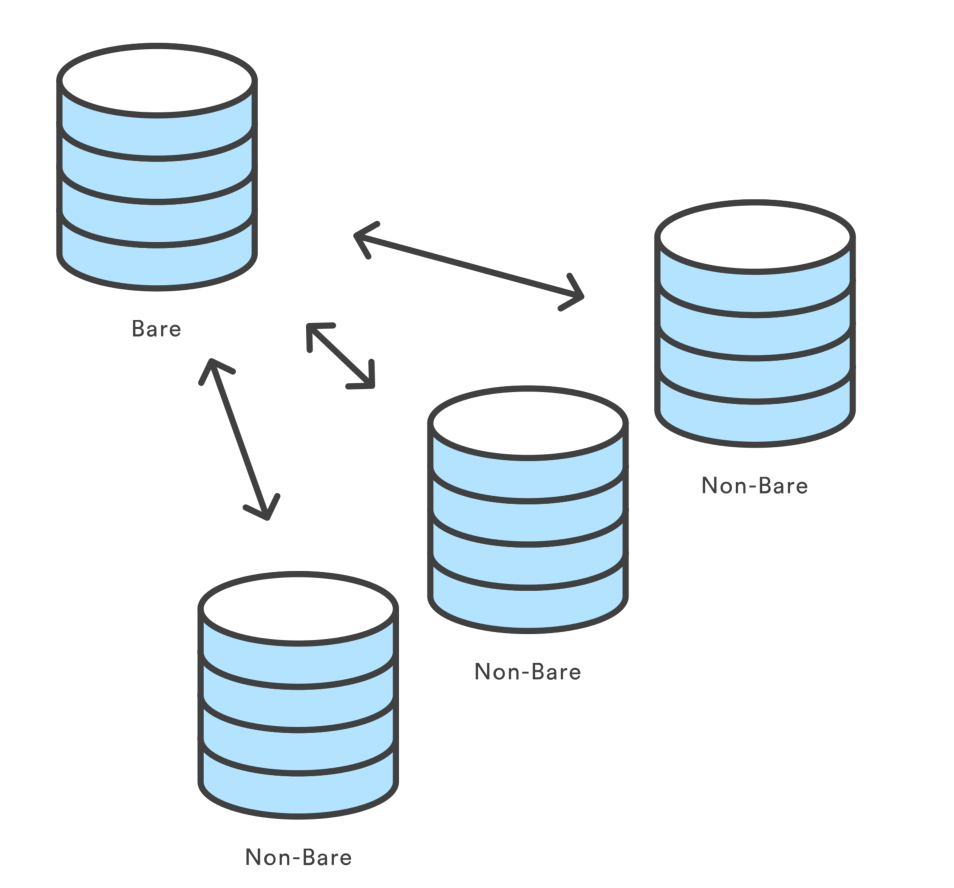
\includegraphics[scale=0.5]{figures/01.pdf}
\end{center}

\subsubsection*{git clone}

The git clone command copies an existing Git repository.

\begin{lstlisting}
$ git clone <repo> <directory>
\end{lstlisting}
Clone the repository located at <repo> url into the folder called
<directory> on the local machine. If <directory> parameter is omitted
the current working directory is used. 

If a project has already been set up in a central repository, the git
clone command is the most common way for users to obtain a development
copy.

Unlike SVN, Git makes no distinction between the working copy and the
central repository - they are all full-fledged Git repositories.
Git's collaboration model is based on repository-to-repository
interaction. Instead of checking a working copy into SVN's central
repository, you push or pull commits from one repository to another.

\begin{center}
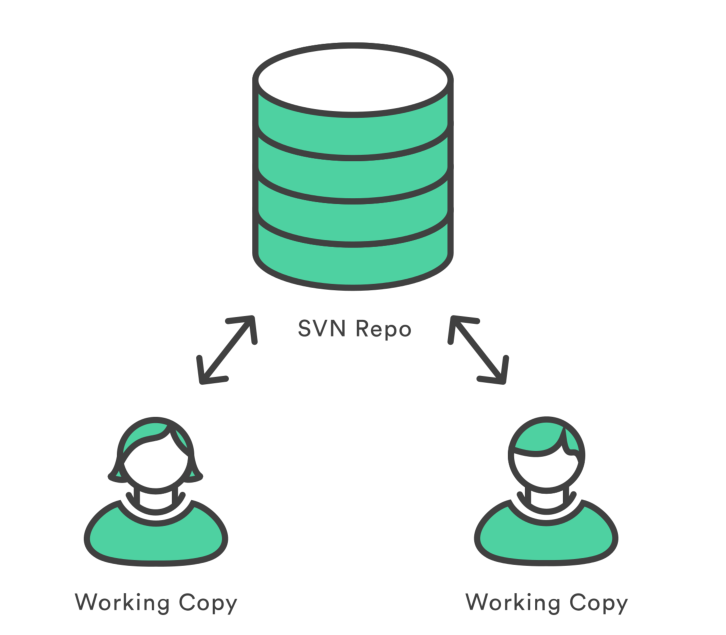
\includegraphics[scale=0.5]{figures/02.pdf}
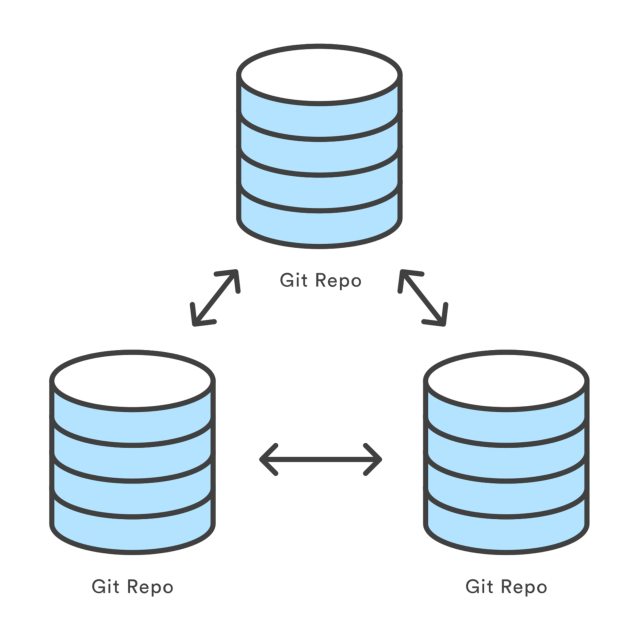
\includegraphics[scale=0.5]{figures/03.pdf}
\end{center}

Of course, there's nothing stopping you from giving certain Git repos
special meaning. For example, in the course one Git repo is going to be
considered as the “central” repository, but this is just a matter of
convention.

\subsubsection*{git config}

Define the author name and email to be used for all commits in the current
repository. Typically, you'll want to use the --global flag to set
configuration options for the current user.

\begin{lstlisting}
$ git config --global user.name "John Smith"
$ git config --global user.email john@example.com 
\end{lstlisting}

\subsection{Saving and reading changes}

The git add and git commit commands compose the fundamental Git
workflow. These are the two commands that every Git user needs to
understand, regardless of their team's collaboration model. They are
the means to record versions of a project into the repository's
history. Finally, git checkout is used to browse any of the previous
commits.

\subsubsection*{git add}

The git add command adds a change in the working directory to the
staging area. It tells Git that you want to include updates to a
particular file in the next commit. 

\begin{lstlisting}
$ git add <file or directory> 
\end{lstlisting}

\begin{lstlisting}
$ git reset <file or directory> 
\end{lstlisting}

With git reset commant you can revert the git add commant.

\subsubsection*{git commit}

However, git add doesn't really
affect the repository in any significant way - changes are not actually
recorded until you run git commit. 

For each commit git asks for a mandatory message that needs to explain
what are the changes that are introduced from the stage to the repository. 

\begin{lstlisting}
$ git commit -m "<message>"
\end{lstlisting}

Developing a project revolves around the basic edit/stage/commit
pattern. First, you edit your files in the working directory. When
you're ready to save a copy of the current state of the project, you
stage changes with git add. After you're happy with the staged
snapshot, you commit it to the project history with git commit. 

\begin{center}
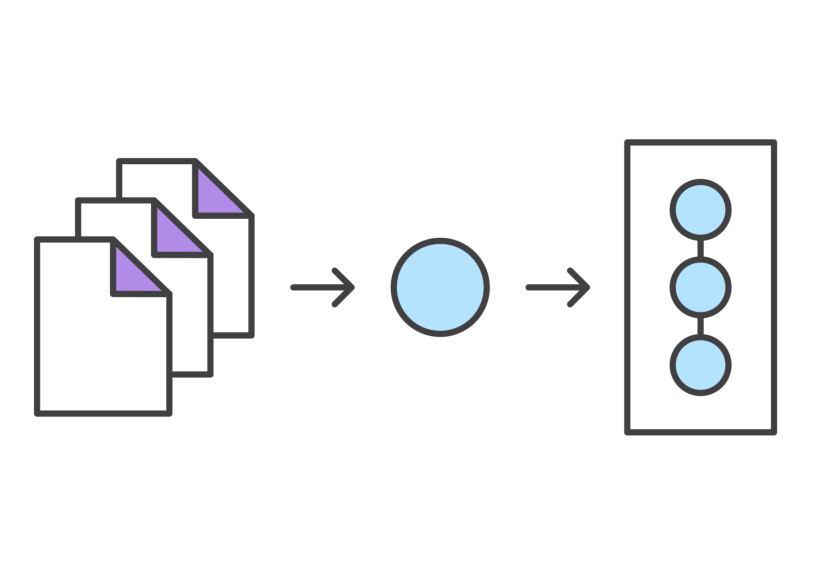
\includegraphics[scale=0.5]{figures/04.pdf}
\end{center}

Instead of committing all of the changes you've made since the last
commit, the stage lets you group related changes into highly focused
snapshots before actually committing it to the project history. This
means you can make all sorts of edits to unrelated files, then go back
and split them up into logical commits by adding related changes to
the stage and commit them piece-by-piece. As in any revision control
system, it's important to create atomic commits so that it's easy to
track down bugs and revert changes with minimal impact on the rest of
the project. 

Commit a snapshot of all changes in the working directory. This only
includes modifications to tracked files (those that have been added
with git add at some point in their history).

Snapshots are always committed to the local repository. Git doesn't
force you to interact with the central repository until you're
ready. Just as the staging area is a buffer between the working
directory and the project history, each developer's local repository
is a buffer between their contributions and the central repository.

\subsubsection*{git checkout}

The git checkout command serves three distinct functions: checking out
files, checking out commits, and checking out branches. In this
section, we will focus more on the first two.

Checking out a commit makes the entire working directory match that
commit. This can be used to view an old state of your project without
altering your current state in any way. Checking out a file lets you
see an old version of that particular file, leaving the rest of your
working directory untouched.

\begin{lstlisting}
$ git checkout <branch name>
\end{lstlisting}

This command changes the current branch in the repository and navigate
the current working directory to the last (head) commit in the branch.

\begin{lstlisting}
$ git checkout <commit ID> <file>
\end{lstlisting}
Check out a previous version of a file. This turns the <file> that
resides in the working directory into an exact copy of the one from
<commit> and adds it to the staging area.

\begin{lstlisting}
$ git checkout <commit ID>
\end{lstlisting}

Update all files in the working directory to match the specified
commit. You can use either a commit hash or a tag as the <commit>
argument. This will put you in a so called detached HEAD state.

\subsection{Inspecting a repository}

In conjunction with add and commit commands, you'll also need git status to
view the state of the working directory and the staging area as well
as git log to view committed snapshots.

\begin{lstlisting}
$ git status
$ git log
\end{lstlisting}

\begin{center}
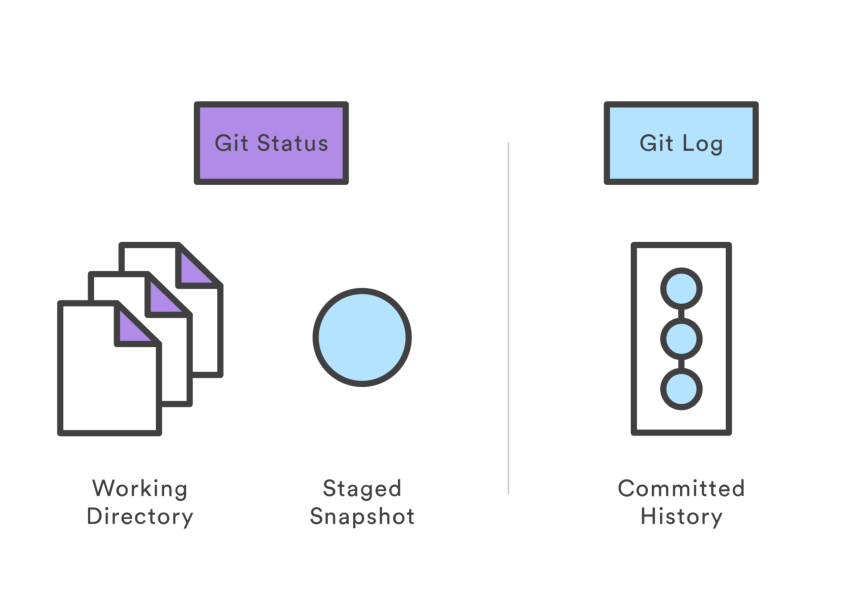
\includegraphics[scale=0.5]{figures/05.pdf}
\end{center}

\textbf{Example (Modifying and inspecting local repository):}
\begin{lstlisting}
$ git init MyRepo
$ cd MyRepo
$ touch Test.java
$ git status
On branch master

Initial commit

Untracked files:
  (use "git add <file>..." to include in what will be committed)

	Test.java

nothing added to commit but untracked files present (use "git add" to
track)
$ git add Test.java 
$ git status
On branch master

Initial commit

Changes to be committed:
  (use "git rm --cached <file>..." to unstage)

	new file:   Test.java

$ git reset Test.java
$ git add Test.java
$ git commit -m "Added Test.java file"
[master (root-commit) 722c655] Added Test.java file
 1 file changed, 0 insertions(+), 0 deletions(-)
 create mode 100644 Test.java
$ git log
commit 722c65503b8109195a0aa1da87644b9e1e45600b
Author: Srdjan Krstic <krledmno1@gmail.com>
Date:   Thu Jan 15 16:35:57 2015 +0100

    Added Test.java file

$ echo "public class Test { }" > Test.java
$ git status
On branch master
Changes not staged for commit:
  (use "git add <file>..." to update what will be committed)
  (use "git checkout -- <file>..." to discard changes in working directory)

	modified:   Test.java

no changes added to commit (use "git add" and/or "git commit -a")
$ git commit -a -m "Written the Test class"
[master 5afb2f7] Written the Test class
 1 file changed, 2 insertions(+)
$ git log --oneline
5afb2f7 Written the Test class
722c655 Added Test.java file
$ git checkout 722c655
Note: checking out '722c655'.
HEAD is now at 722c655... Added Test.java file
$ git status
HEAD detached at 722c655
nothing to commit, working directory clean
$ git checkout master
Previous HEAD position was 722c655... Added Test.java file
Switched to branch 'master'
$ git log --oneline
5afb2f7 Written the Test class
722c655 Added Test.java file
\end{lstlisting}

\subsection{Branching}

Git can keep history that is non-linear. Developers can create several
branches in their project revision history and use them to develop
separate features in isolated environment. 
To perform branching in git first one needs to know how to create branches. 
Then, as we mentioned before, we'll see how git checkout can be used to
select a branch. Finally, we'll learn how git merge can integrate the
history of independent branches.

\subsubsection*{git branch}

A branch represents an independent line of development.
 You can think of them as a
way to request a brand new working directory, staging area, and
project history. New commits are recorded in the history for the
current branch, which results in a fork in the history of the
project.

The git branch command lets you create, list, rename, and delete
branches.

\begin{lstlisting}
$ git branch
\end{lstlisting}

Lists all the branches in your repository.

\begin{lstlisting}
$ git branch <name>
\end{lstlisting}

Creates a new branch called <name>. This does not check out the new
branch (i.e. it does not make it current branch).

\begin{lstlisting}
$ git branch -d <name>
\end{lstlisting}

Deletes the specified branch.

\begin{lstlisting}
$ git branch -m <name>
\end{lstlisting}

Renames the current branch to <name>.

 Branches should be a part of your everyday development
 process. When you want to add a new feature or fix a bug - no matter
 how big or how small - you spawn a new branch to encapsulate your
 changes. This makes sure that unstable code is never committed to the
 main code base.

\subsubsection*{git checkout}

The git checkout command lets you navigate between the branches
created by git branch. Checking out a branch updates the files in the
working directory to match the version stored in that branch, and it
tells Git to record all new commits on that branch. Think of it as a
way to select which line of development you're working on.

\begin{lstlisting}
$ git checkout <existing branch name>
\end{lstlisting}

Check out the specified branch, which should have already been
created.

git checkout works hand-in-hand with git branch. When you want to
start a new feature, you create a branch with git branch, then check
it out with git checkout. You can work on multiple features in a
single repository by switching between them with git checkout. 

Remember that the HEAD is Git's way of referring to the current
snapshot. Internally, the git checkout command simply updates the HEAD
to point to either the specified branch or commit. When it points to a
branch, Git doesn't complain, but when you check out a commit, it
switches into a ``detached HEAD'' state.

\begin{center}
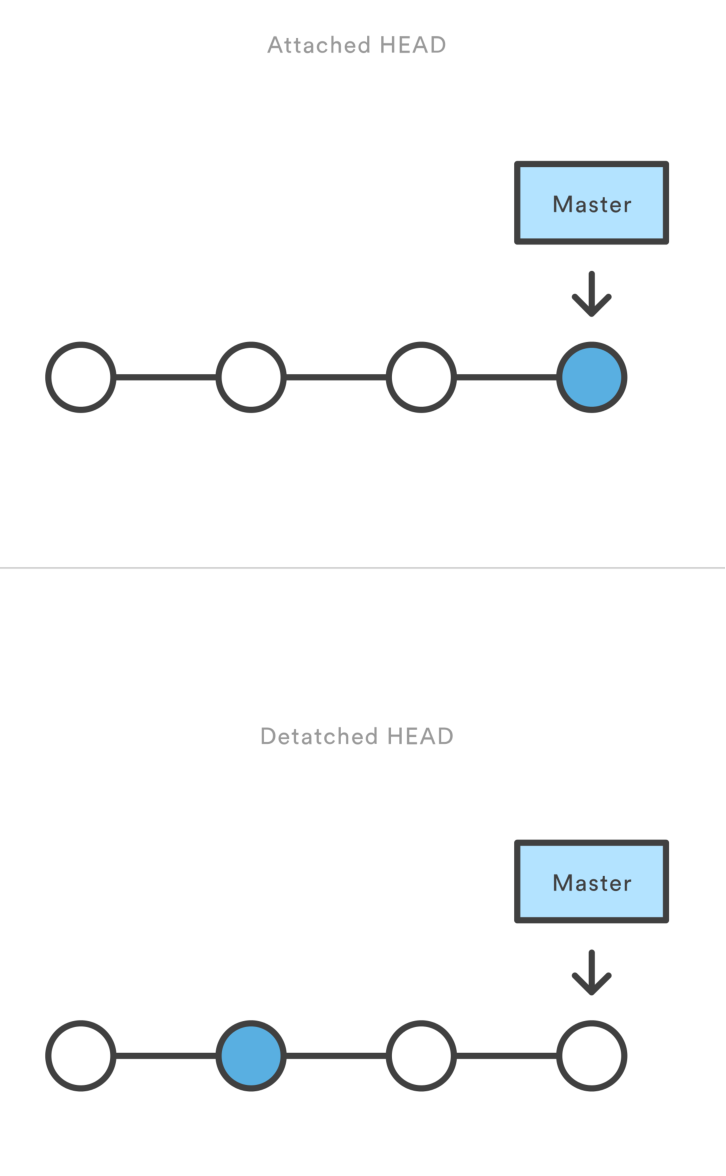
\includegraphics[scale=0.5]{figures/09.pdf}
\end{center}

This is a warning telling you that everything you're doing is
``detached'' from the rest of your project's development. If you were to
start developing a feature while in a detached HEAD state, there would
be no branch allowing you to get back to it. When you inevitably check
out another branch (e.g., to merge your feature in), there would be no
way to reference your feature. The point is, your development should
always take place on a branch - never on a detached HEAD. 

\subsubsection*{git merge}

Merging is Git's way of putting a forked history back together
again. The git merge command lets you take the independent lines of
development created by git branch and integrate them into a single
branch. 

Note that all of the commands presented below merge into the current
branch. The current branch will be updated to reflect the merge, but
the target branch will be completely unaffected. Again, this means
that git merge is often used in conjunction with git checkout for
selecting the current branch and git branch -d for deleting the
obsolete target branch.

\begin{lstlisting}
$ git merge <existing branch name>
\end{lstlisting}

Merge the specified branch into the current branch. Git will determine
the merge algorithm automatically (discussed below). 

\begin{lstlisting}
$ git merge --no-ff <existing branch name>
\end{lstlisting}

Merge the specified branch into the current branch, but always
generate a merge commit (even if it was a fast-forward merge). This is
useful for documenting all merges that occur in your repository.

Once you've finished developing a feature in an isolated branch, it's
important to be able to get it back into the main code base. Depending
on the structure of your repository, Git has several distinct
algorithms to accomplish this: a fast-forward merge or a 3-way merge. 

A fast-forward merge can occur when there is a linear path from the
current branch tip to the target branch. Instead of ``actually'' merging
the branches, all Git has to do to integrate the histories is move
(i.e., ``fast forward'') the current branch tip up to the target branch
tip. This effectively combines the histories, since all of the commits
reachable from the target branch are now available through the current
one. For example, a fast forward merge of some-feature into master
would look something like the following: 

\begin{center}
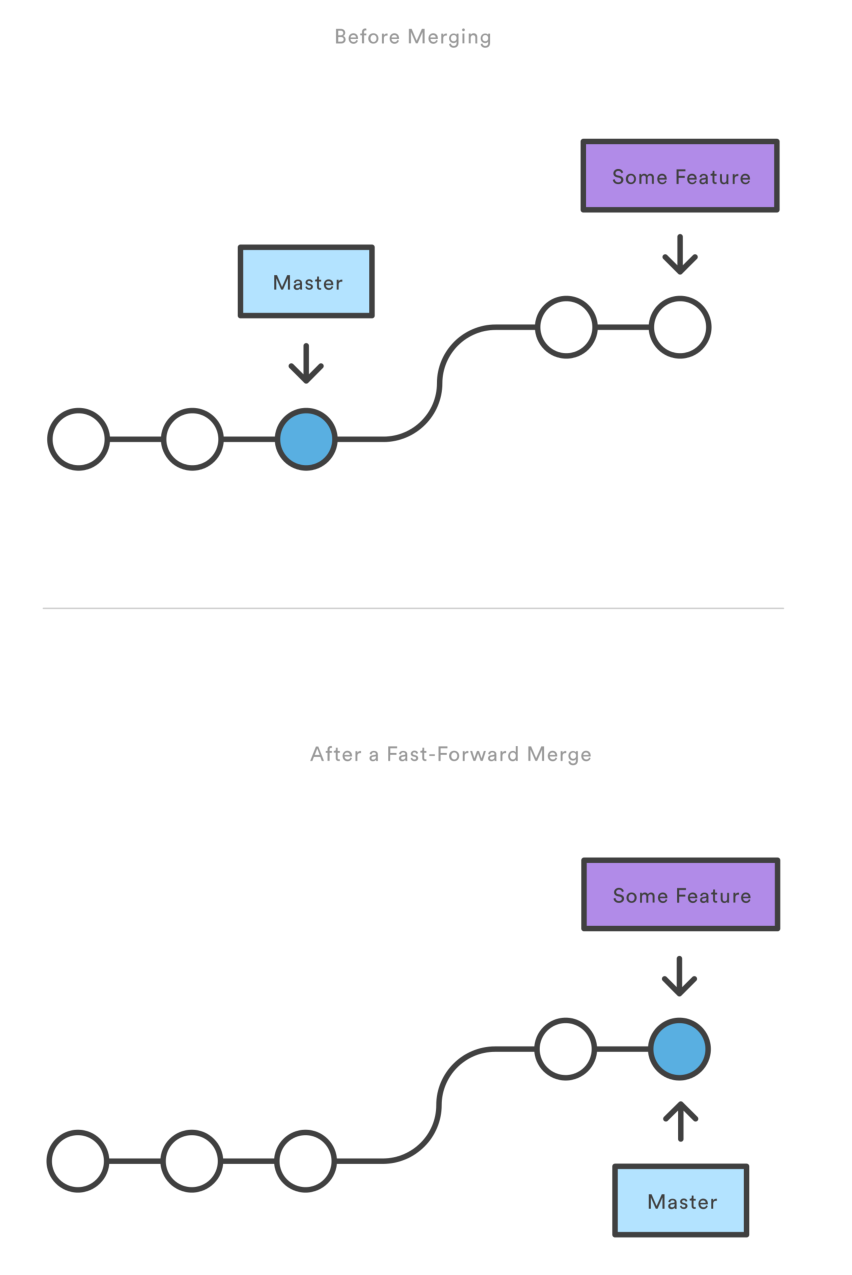
\includegraphics[scale=0.5]{figures/10.pdf}
\end{center}

However, a fast-forward merge is not possible if the branches have
diverged. When there is not a linear path to the target branch, Git
has no choice but to combine them via a 3-way merge. 3-way merges use
a dedicated commit to tie together the two histories. The nomenclature
comes from the fact that Git uses three commits to generate the merge
commit: the two branch tips and their common ancestor. 

While you can use either of these merge strategies, many developers
like to use fast-forward merges (facilitated through rebasing) for
small features or bug fixes, while reserving 3-way merges for the
integration of longer-running features. In the latter case, the
resulting merge commit serves as a symbolic joining of the two
branches. 

\begin{center}
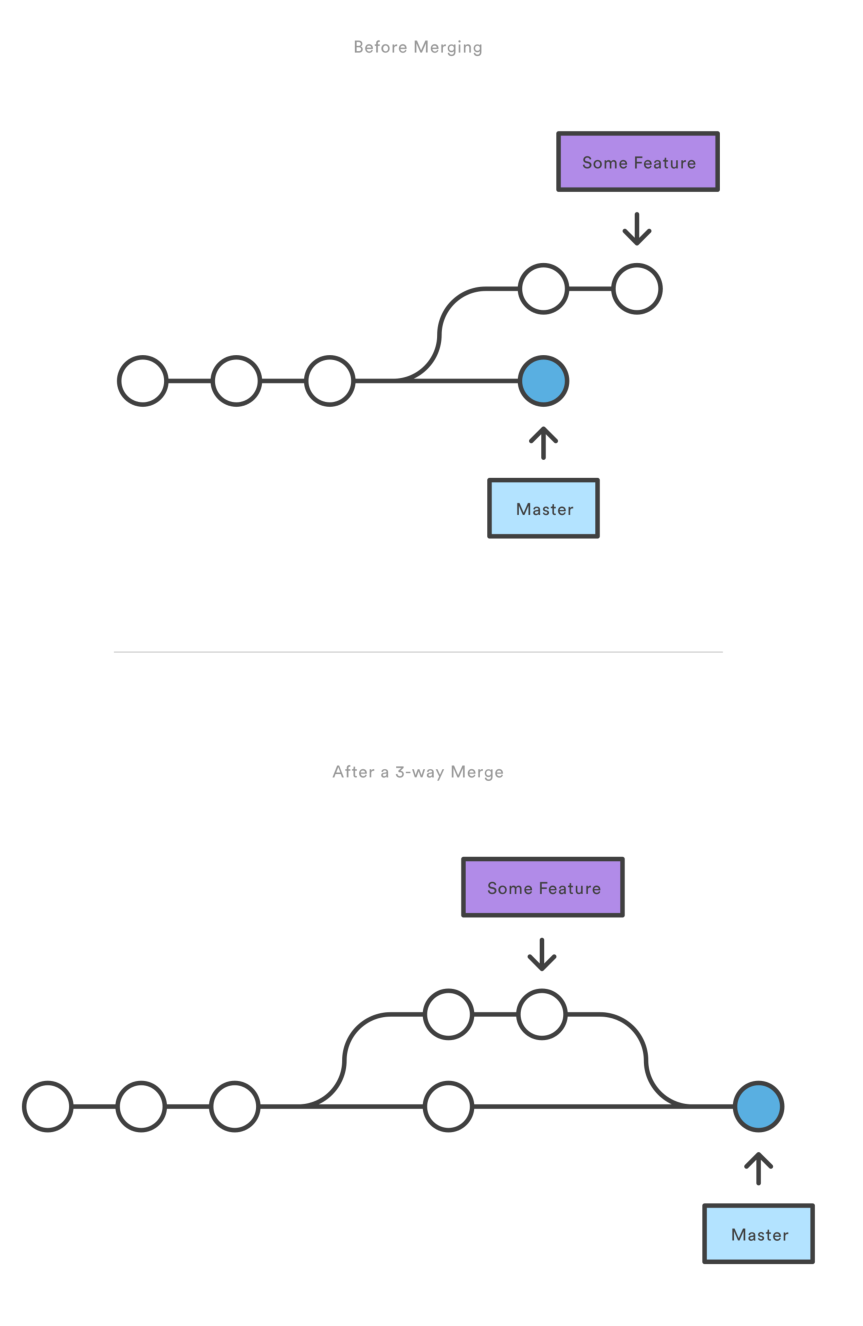
\includegraphics[scale=0.5]{figures/11.pdf}
\end{center}



If the two branches you're trying to merge both changed the same part
of the same file, Git won't be able to figure out which version to
use. When such a situation occurs, it stops right before the merge
commit so that you can resolve the conflicts manually. 
When you encounter a merge conflict, running the git status command
shows you which files need to be resolved. 

Then, you can go in and fix up the merge to your liking. When you're
ready to finish the merge, all you have to do is run git add on the
conflicted file(s) to tell Git they're resolved. Then, you run a
normal git commit to generate the merge commit. 


\textbf{Example (Creating and merging branches):}\\
Continues from the previous example
\begin{lstlisting}
$ git branch
* master
$ git branch experimental
$ git branch
  experimental
* master
$ git checkout experimental
Switched to branch 'experimental'
$ echo "public class Experiment { }" > Experiment.java
$ git add Experiment.java
$ git commit  -m "Added experimental feature"
[experimental 641495a] Added experimental feature
 1 file changed, 1 insertion(+)
 create mode 100644 Experiment.java
$ ls
Experiment.java	Test.java
$ git checkout master
Switched to branch 'master'
$ ls
Test.java
$ git merge experimental
Updating 5afb2f7..641495a
Fast-forward
 Experiment.java | 1 +
 1 file changed, 1 insertion(+)
 create mode 100644 Experiment.java
$ ls
Experiment.java	Test.java
$ git branch -d experimental
Deleted branch experimental (was 641495a).
$ git branch
* master
$ git branch feature
$ git checkout feature
Switched to branch 'feature'
$ echo "public class Experiment { int a; }" > Experiment.java
$ git add Experiment.java
$ git commit  -m "Added variable a"
[feature 80ba1c7] Added variable a
 1 file changed, 1 insertion(+), 1 deletion(-)
$ git checkout master
Switched to branch 'master'
$ cat Experiment.java
public class Experiment { }
$ echo "public class Experiment { int b; }" > Experiment.java
$ git add Experiment.java
$ git commit  -m "Added variable b"
[master 4aff254] Added variable b
 1 file changed, 1 insertion(+), 1 deletion(-)
$ git merge feature
Auto-merging Experiment.java
CONFLICT (content): Merge conflict in Experiment.java
Automatic merge failed; fix conflicts and then commit the result.
$ cat Experiment.java
<<<<<<< HEAD
public class Experiment { int b; }
=======
public class Experiment { int a; }
>>>>>>> feature
$ echo "public class Experiment { int ab; }" > Experiment.java
$ git add Experiment.java
$ git commit  -m "Added variable ab"
[master b0b4a98] Added variable ab
$ git log --oneline
b0b4a98 Added variable ab
4aff254 Added variable b
80ba1c7 Added variable a
641495a Added experimental feature
5afb2f7 Written the Test class
722c655 Added Test.java file
\end{lstlisting}


\subsection{Synchronizing with remote repositories}

Git's collaboration model gives every developer their own copy
of the repository, complete with its own local history and branch
structure. Instead of committing a changeset from a
working copy to the central repository, Git lets you share entire
branches between repositories. 

The commands presented below let you manage connections with other
repositories, publish local history by ``pushing'' branches to other
repositories, and see what others have contributed by ``pulling''
branches into your local repository.

\begin{center}
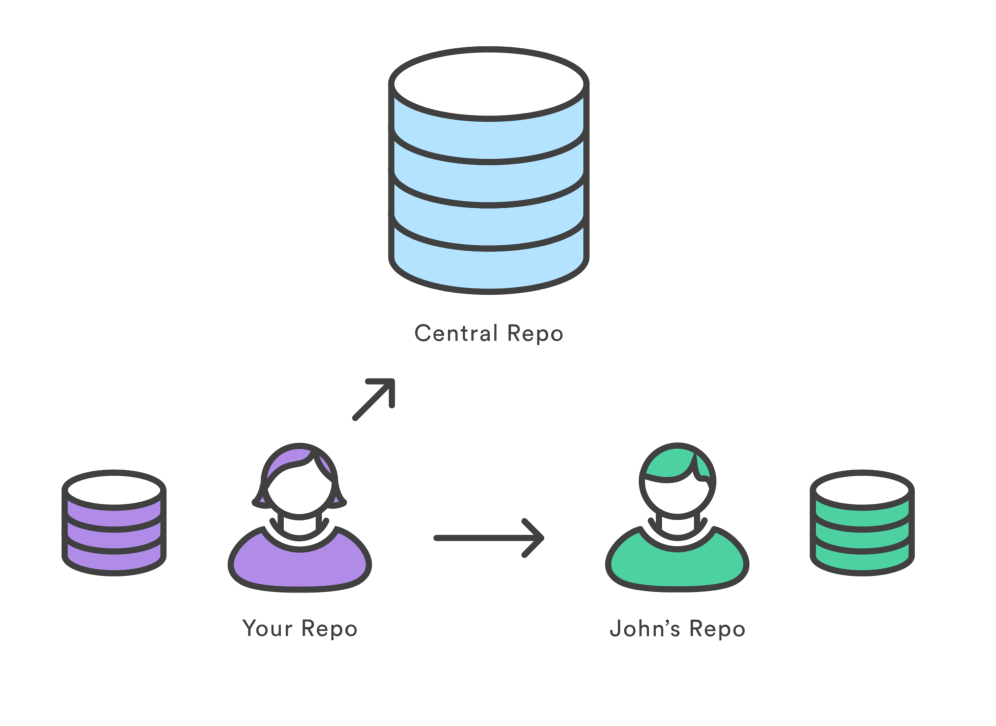
\includegraphics[scale=0.5]{figures/06.pdf}
\end{center}

\subsubsection*{git remote}

The git remote command lets you create, view, and delete connections
to other repositories. Remote connections are more like bookmarks
rather than direct links into other repositories. They associate names
to urls of the remote repositories to serve as convenient aliases
that can be used instead of using urls directly.

\begin{lstlisting}
$ git remote
\end{lstlisting}

List the remote connections you have to other repositories.
When you clone a repository with git clone, it automatically creates a
remote connection called origin pointing back to the cloned
repository. This is useful for developers creating a local copy of a
central repository, since it provides an easy way to pull upstream
changes or publish local commits. This behavior is also why most
Git-based projects call their central repository origin.

\begin{lstlisting}
$ git remote add <name> <url>
\end{lstlisting}

Create a new connection to a remote repository. After adding a remote,
you'll be able to use <name> as a convenient shortcut for <url> in
other Git commands.

\begin{lstlisting}
$ git remote rm <name>
\end{lstlisting}

Remove the connection to the remote repository called <name>.

\subsubsection*{git fetch}

The git fetch command imports commits from a remote repository into
your local repo. The resulting commits are stored as remote branches
instead of the normal local branches that we've been working
with. This gives you a chance to review changes before integrating
them into your copy of the project.

\begin{lstlisting}
$ git fetch <name>
\end{lstlisting}

Fetch all of the branches from the repository <name>. This also downloads all
of the required commits and files from the other repository.

\begin{lstlisting}
$ git fetch <name> <branch>
\end{lstlisting}

Fetch a specific branch <branch> from <name>

Fetching is what you do when you want to see what everybody else has
been working on. Since fetched content is represented as a remote
branch, it has absolutely no effect on your local development
work. This makes fetching a safe way to review commits before
integrating them with your local repository.

Remote branches are just like local branches, except they represent
commits from somebody else's repository. You can check out a remote
branch just like a local one, but this puts you in a detached HEAD
state (just like checking out an old commit). You can think of them as
read-only branches. To view your remote branches, simply pass the -r
flag to the git branch command. Remote branches are prefixed by the
remote repository name they belong to so that you don't mix them up with local
branches.



\subsubsection*{git pull}

Fetch the specified remote's copy of the current branch and
immediately merge it into the local copy. This is the same as git
fetch <name> followed by git merge origin/<current-branch>.

\begin{lstlisting}
$ git pull <name>
\end{lstlisting}

The git pull commant is an easy way to synchronize your local repository with upstream
changes. The following diagram explains each step of the pulling
process in your local revision history: 

\begin{center}
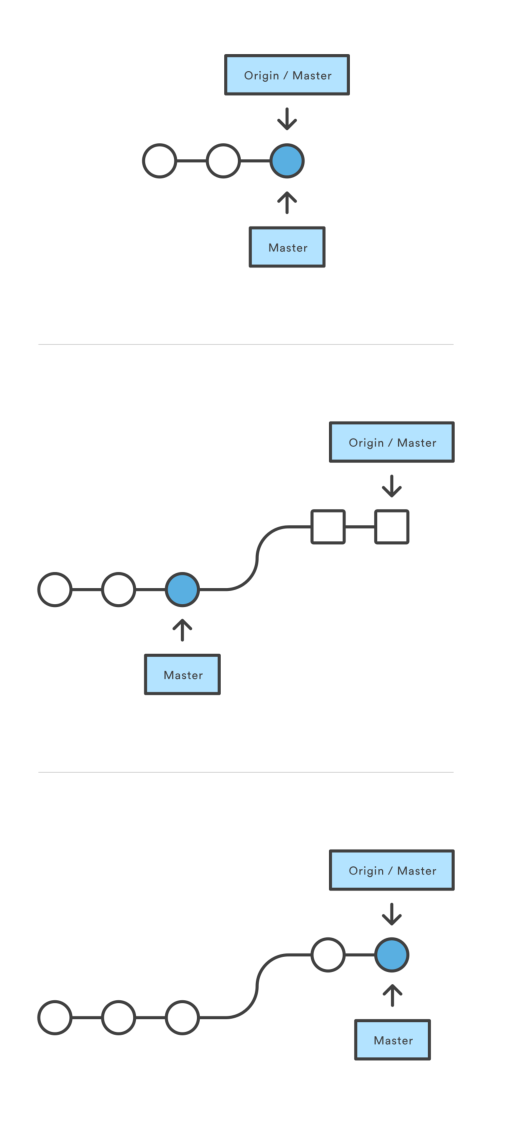
\includegraphics[scale=0.7]{figures/07.pdf}
\end{center}


\subsubsection*{git push}

Pushing is how you transfer commits from your local repository to a
remote repo. It's the counterpart to git fetch, but whereas fetching
imports commits to local branches, pushing exports commits to remote
branches. This has the potential to overwrite changes, so you need to
be careful how you use it. These issues are discussed below.

\begin{lstlisting}
$ git pull <name> <branch>
\end{lstlisting}

Push the specified branch to <name>, along with all of the necessary
commits and internal objects. To prevent you from overwriting commits, Git
won't let you push when it results in a non-fast-forward merge in the
destination repository.

Use for git push in the case of the course project is to publish changes
from your local repository to the central repository. 
After you've accumulated several local
commits and are ready to share them with the rest of the team, you
push them to the central repository.

\begin{center}
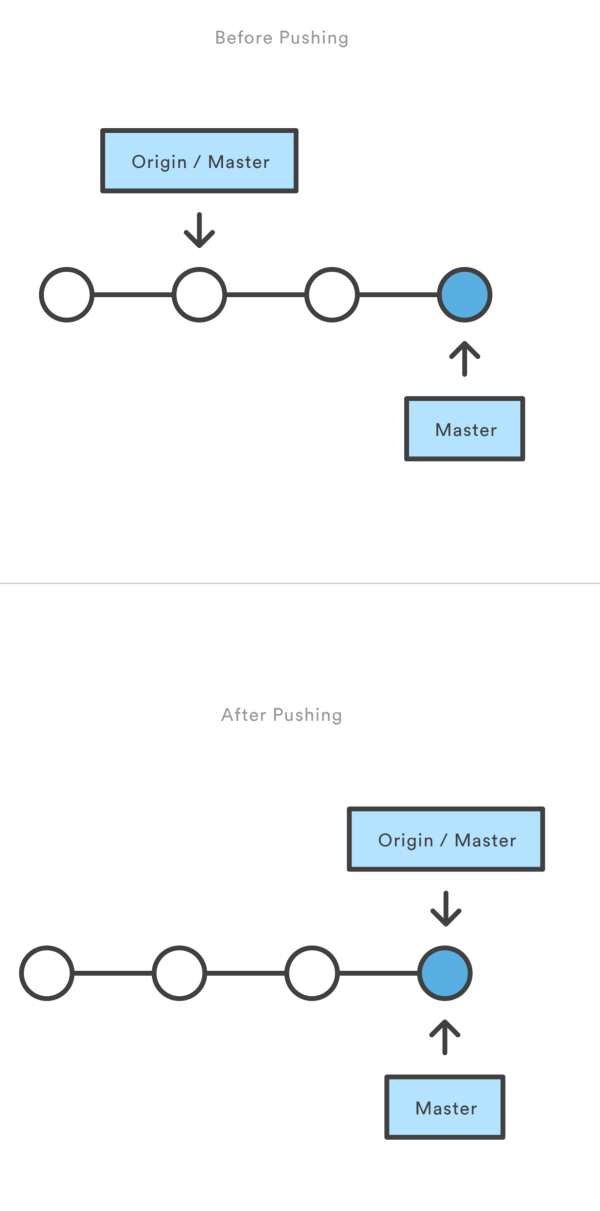
\includegraphics[scale=0.58]{figures/08.pdf}
\end{center}

The above diagram shows what happens when your local master has
progressed past the central repository's master and you publish
changes by running git push origin master. Notice how git push is
essentially the same as running git merge master from inside the
remote repository.

\textbf{Example (Synchronizing with remote repository):}

Set up a remote repository (with bitbucket, for example).
\begin{center}
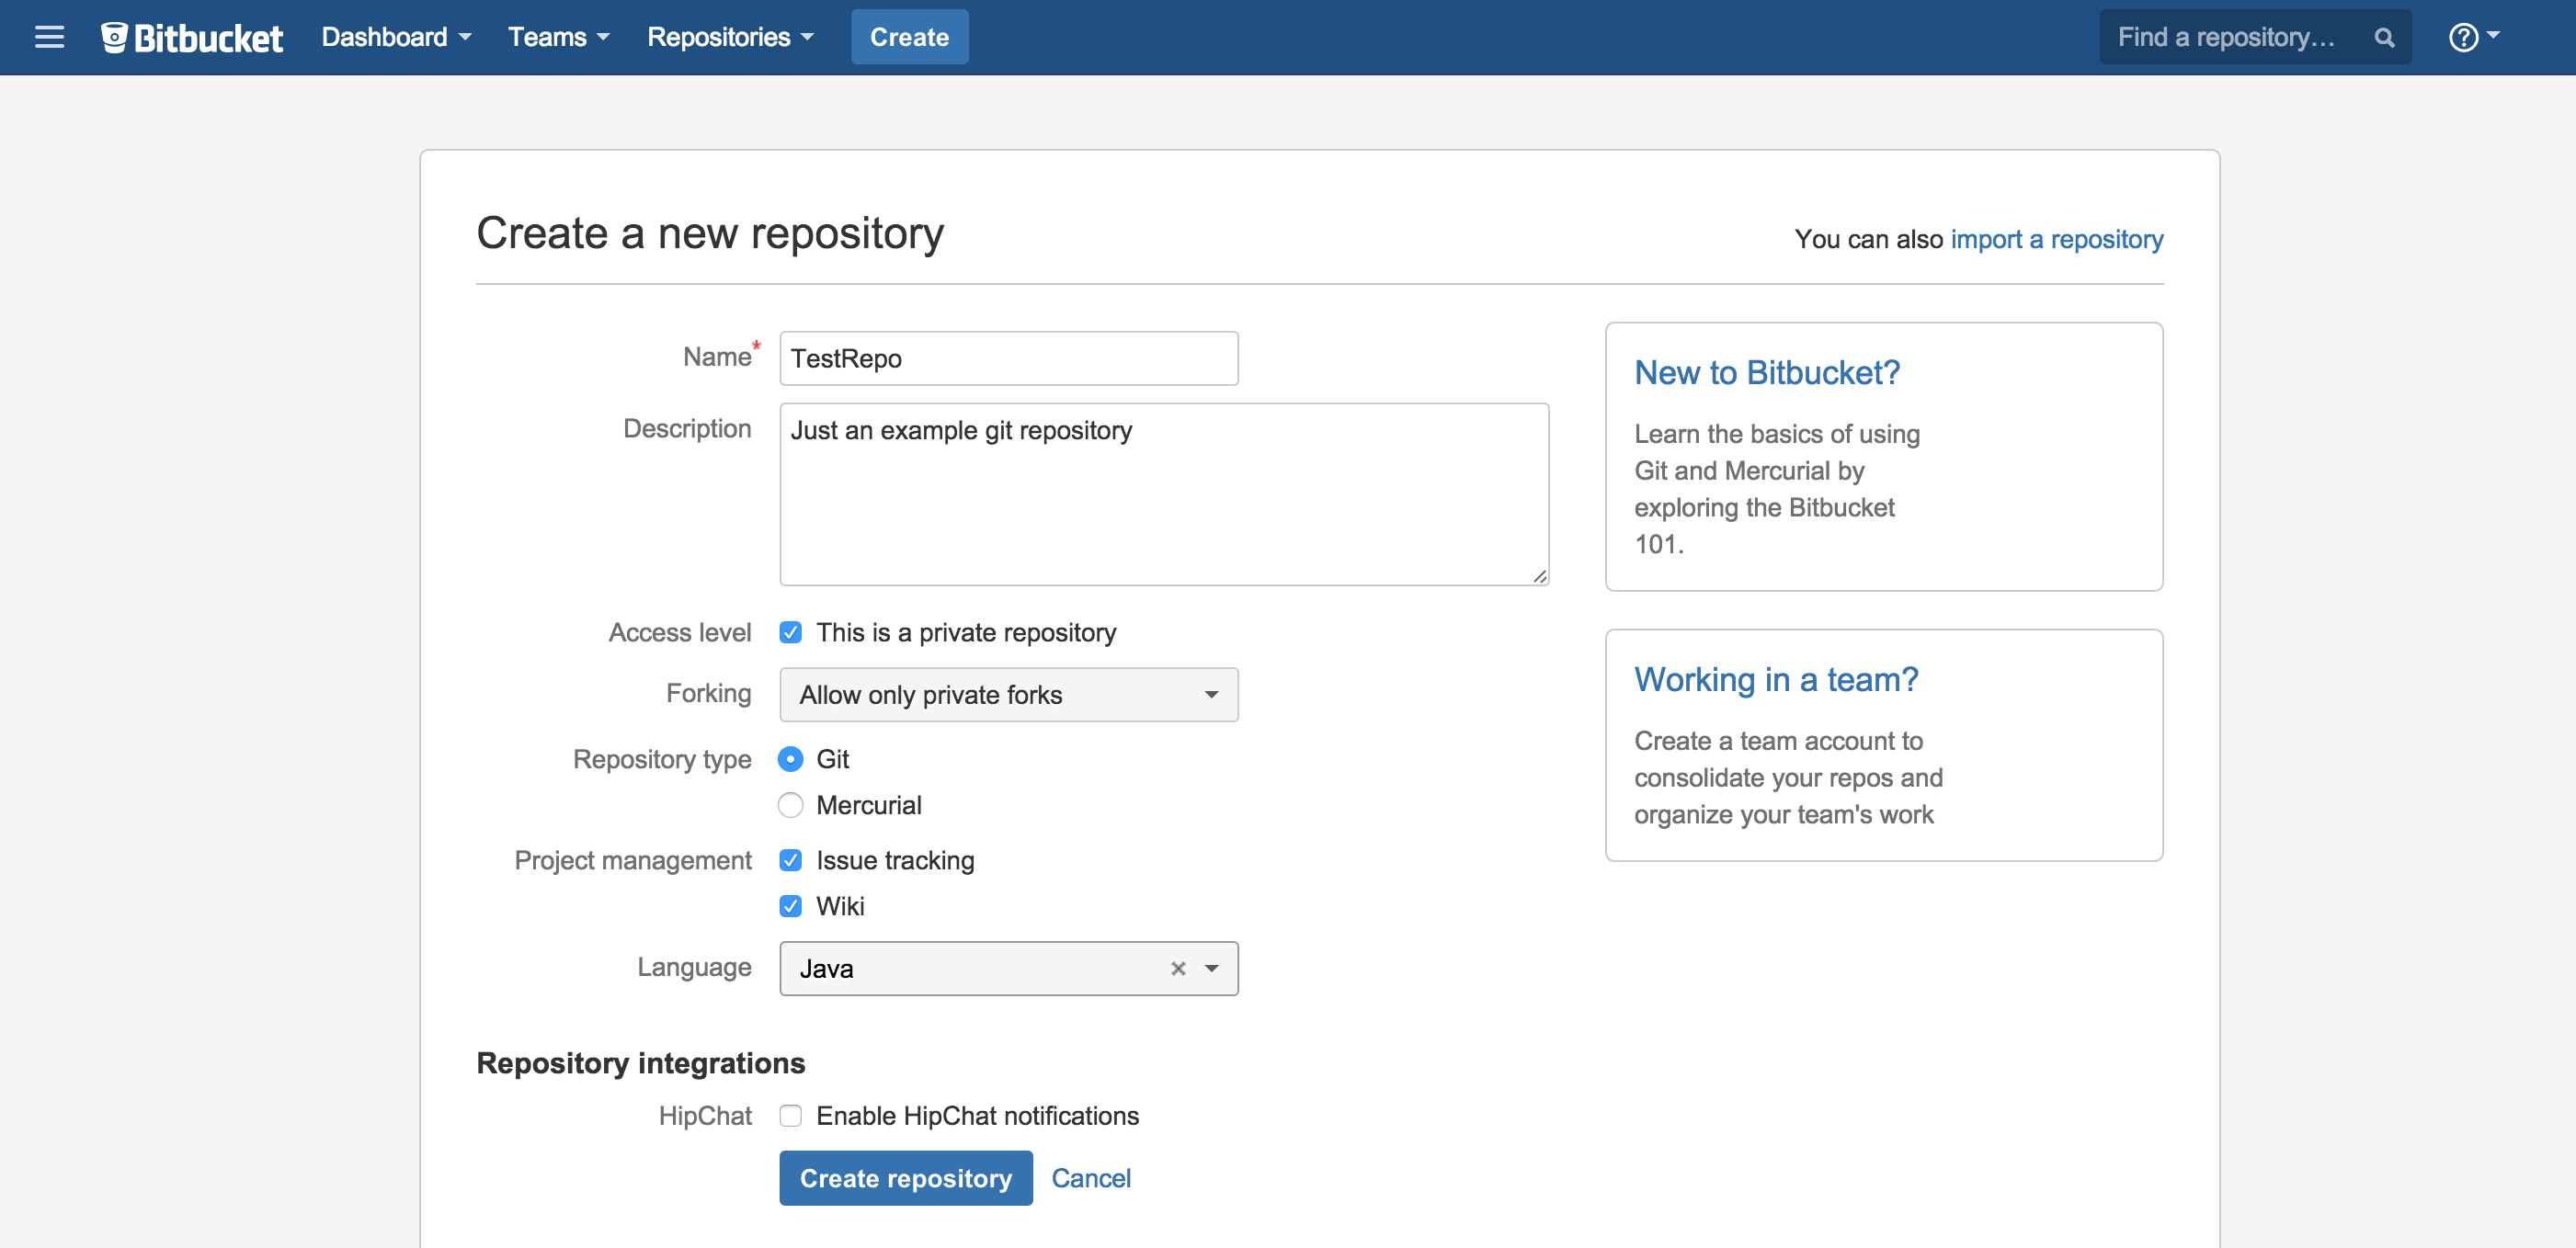
\includegraphics[scale=0.33]{figures/s1.png}
\end{center}

Perform the following set of commands
\begin{lstlisting}
$ git remote add origin https://john@bitbucket.org/john/testrepo.git
$ git remote
origin
$ git push origin
$ git push -u origin --all
Counting objects: 18, done.
Delta compression using up to 8 threads.
Compressing objects: 100% (10/10), done.
Writing objects: 100% (18/18), 1.55 KiB | 0 bytes/s, done.
Total 18 (delta 1), reused 0 (delta 0)
To https://john@bitbucket.org/john/testrepo.git
 * [new branch]      master -> master
Branch master set up to track remote branch master from origin.
$ git pull origin
Already up-to-date.
\end{lstlisting}

You will be able to see all your branches and within each branch all
the commits. In this case there is only the master branch with 6 commits.
\begin{center}
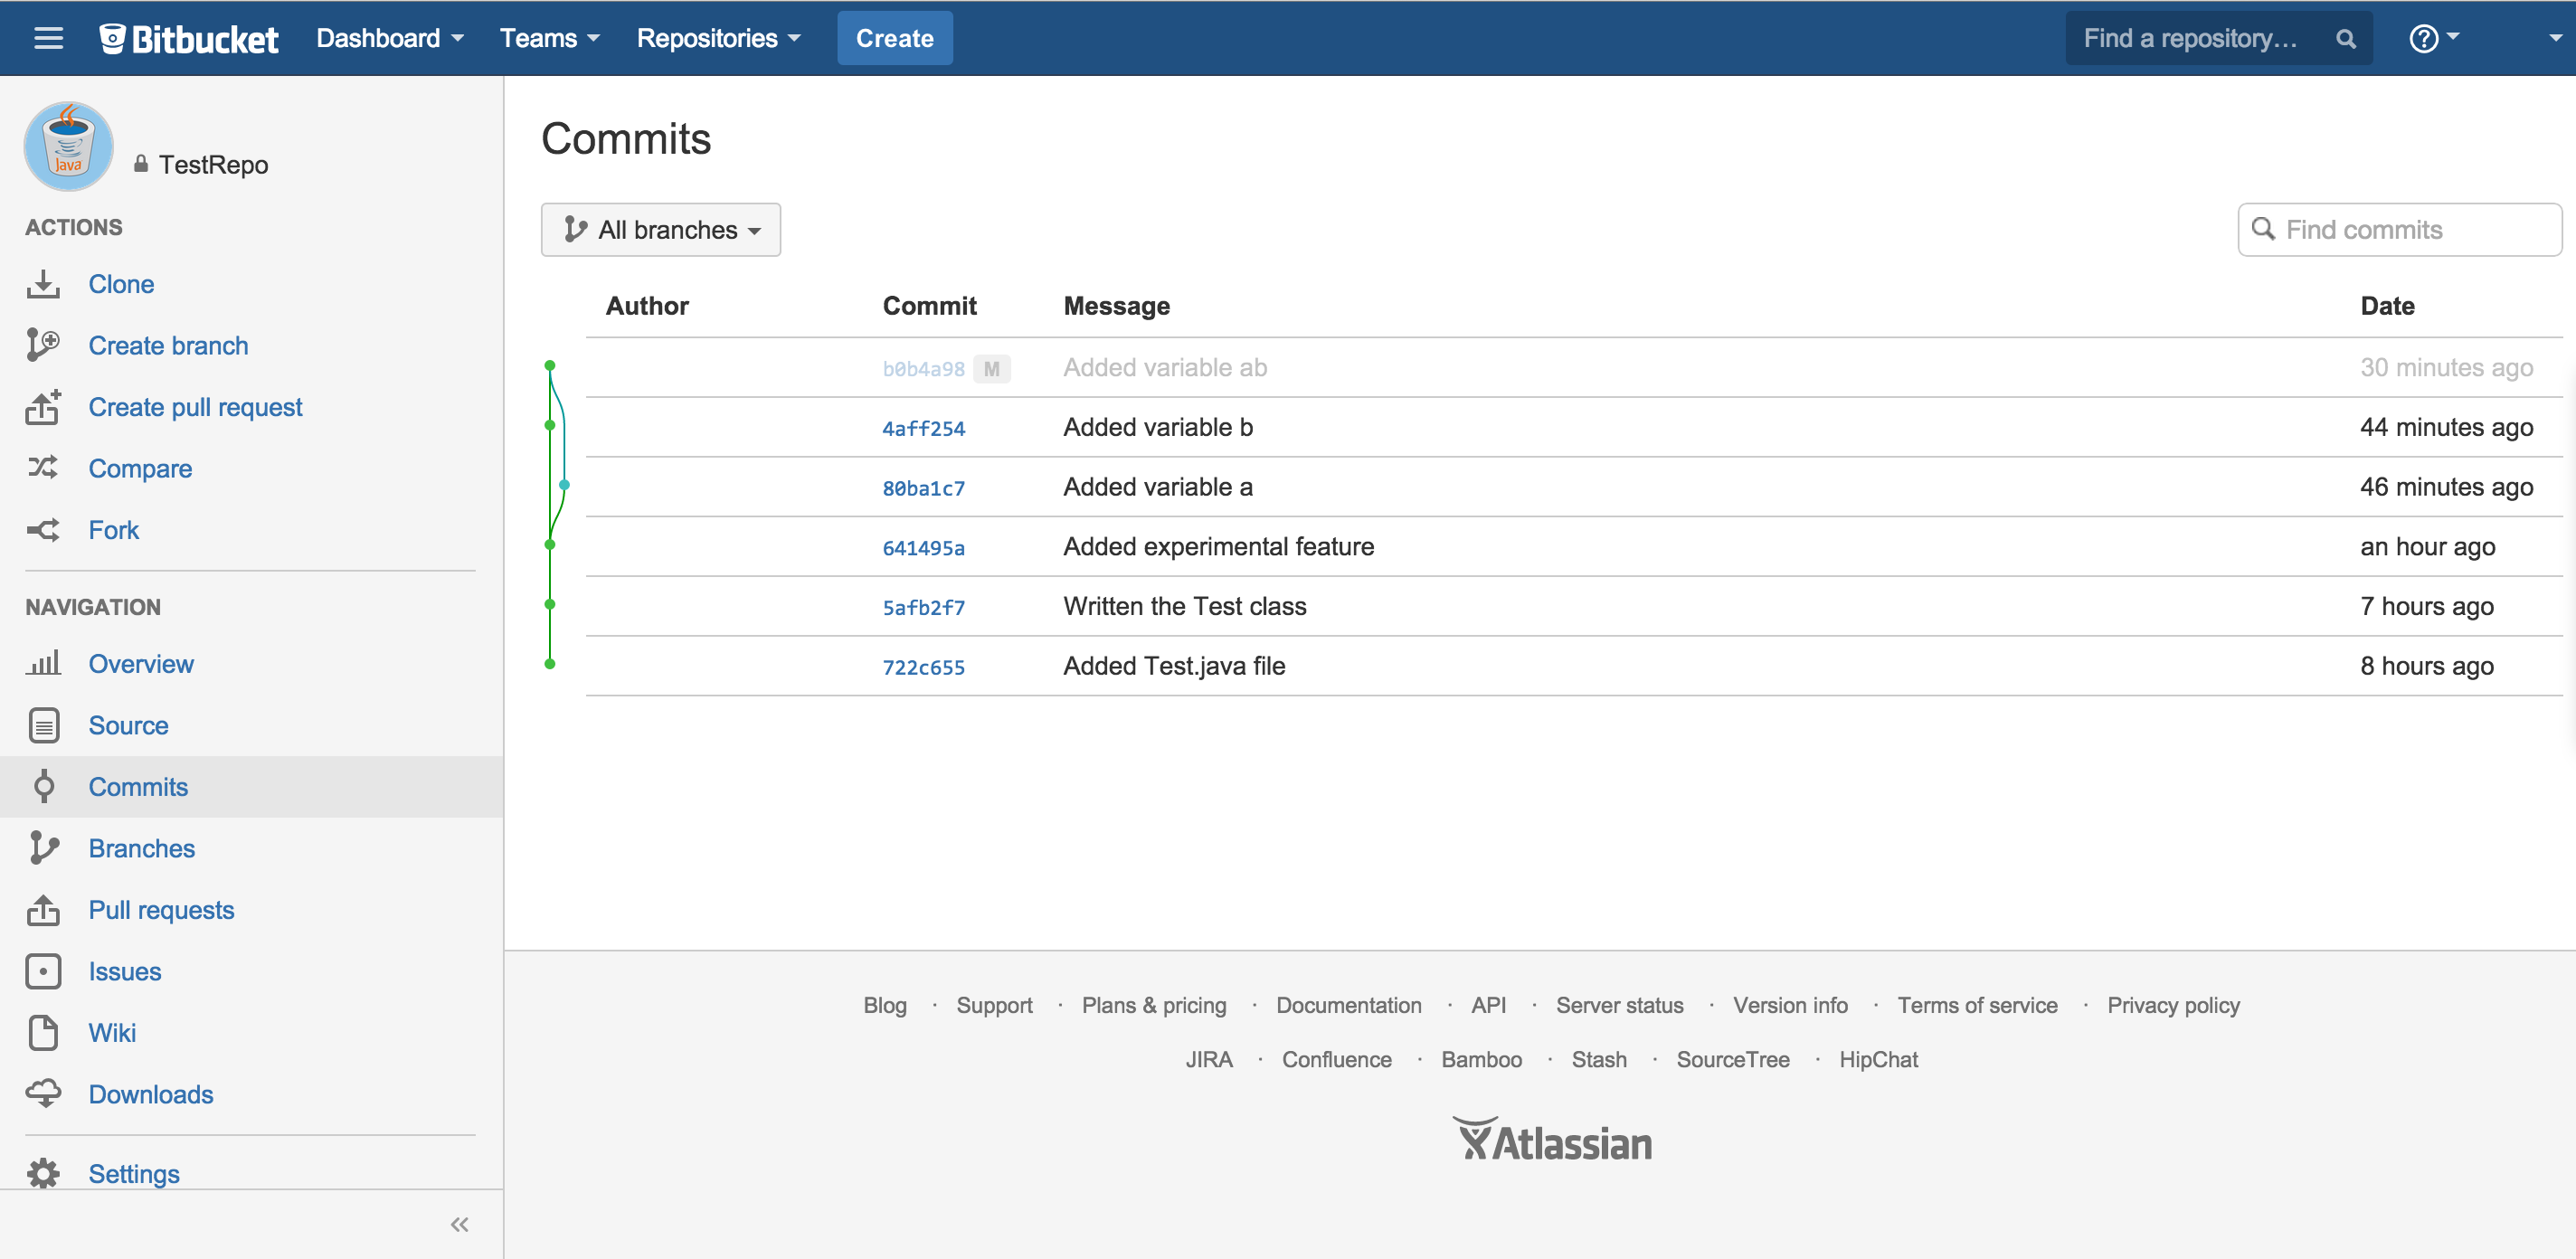
\includegraphics[scale=0.33]{figures/s2.png}
\end{center}

\section{Git with Eclipse}

EGit is an Eclipse plug-in (software component) which allows you to
use the distributed version control system Git directly within the
Eclipse IDE. 

\subsection{Installation}
Eclipse Luna, IDE that we are going to use in the class already contains
EGit 3.4.1, therefore no installation is required. If you decide to
use some other IDE or an older version of Eclipse you need to install
it on your own.
The EGit plug-in can be installed into every Eclipse IDE
installation. Usually EGit supports the last two Eclipse releases.

\subsection{Configuration}

Before using Git you must configure your name and email address which
is used to fill the author and committer information of commits you
create. 

The Git configuration settings can be adjusted via the Eclipse
preference setting. 
Select \\
Window $\rightarrow$ Preferences $\rightarrow$ Team
$\rightarrow$ Git $\rightarrow$ Configuration  (for Windows or Linux)
or\\
Eclipse $\rightarrow$ Preferences $\rightarrow$ Team
$\rightarrow$ Git $\rightarrow$ Configuration (for Mac)\\
to see the current configuration and to change it. 

\begin{center}
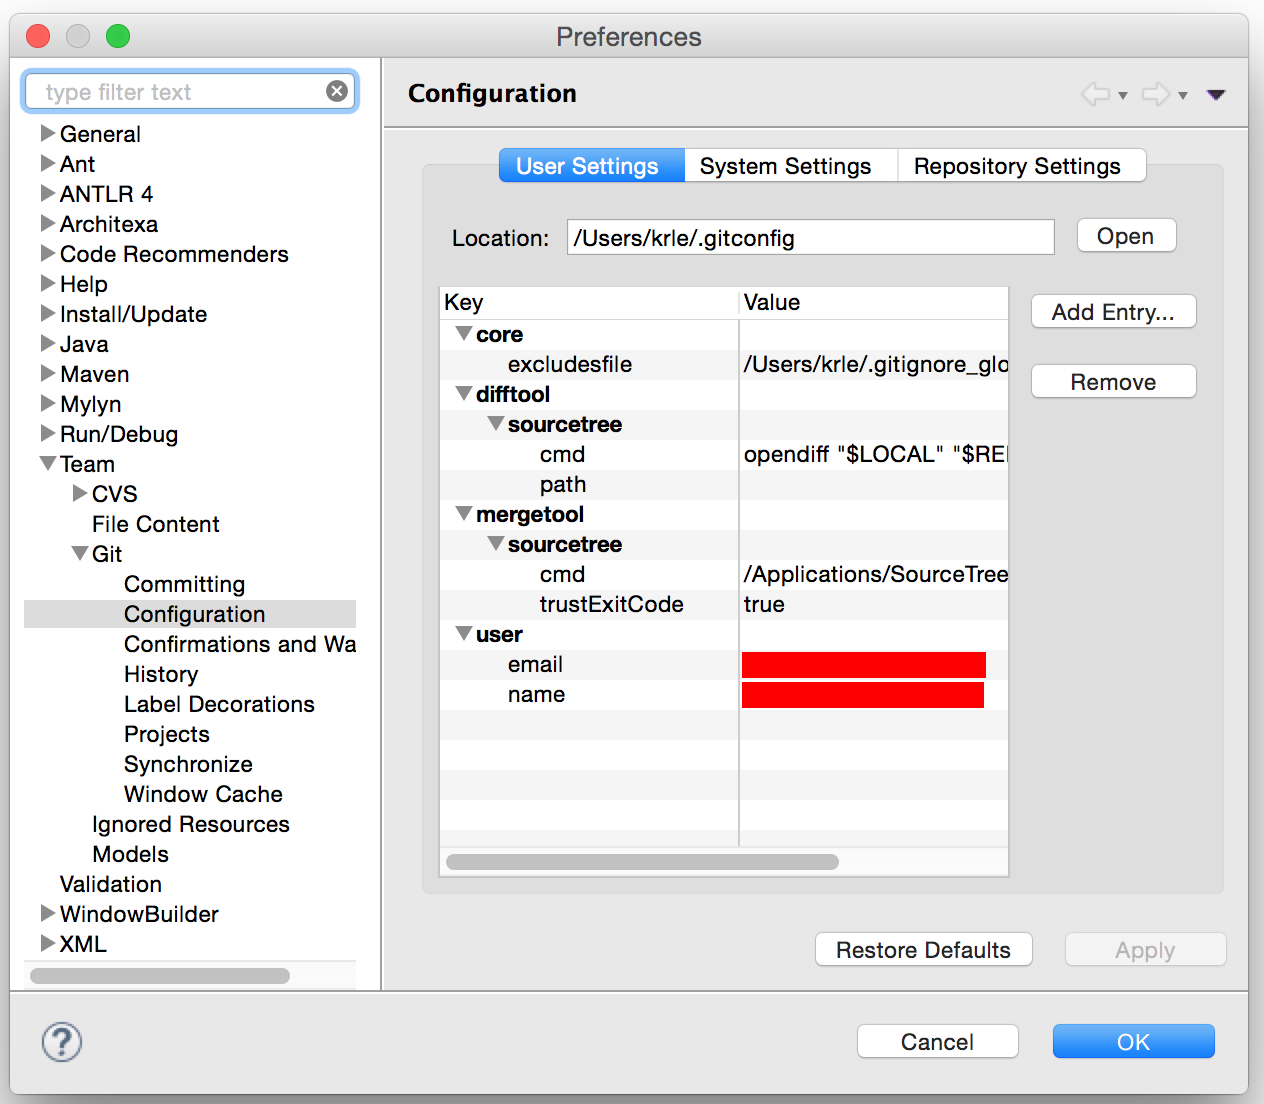
\includegraphics[scale=0.5]{figures/s3.png}
\end{center}

You can add entries to your Git configuration by pressing the Add
Entries button on the Git Configuration preference page. To add your
user, use the user.name as key and your real name as value. Repeat the
procedure for your email address. 

Optionally, you can configure the default folder for storing Git
repositories at the\\ 
Window $\rightarrow$ Preferences $\rightarrow$ Git $\rightarrow$ Team
$\rightarrow$ Default Repository Folder entry (for Windows or Linux) or\\
Eclipse $\rightarrow$ Preferences $\rightarrow$ Git $\rightarrow$ Team
$\rightarrow$ Default  Repository Folder entry (for Mac). 



\subsection{Create new project}

The following section explains how to create a local Git repository
for one project with Eclipse. Having a local repository allows you to keep track of your
changes in the project and allows you to revert to another state at a
later point in time.
 
After that, it will explain how to push all the changes into an empty
remote repository. In the case of the course project, material in this
section can be applied by one team member that can carefully set up a
maven project and the .gitignore file and perform an initial push.

\begin{enumerate}
\item Create a new maven project and set up pom.xml file (refer to the Maven guide)
\item Create a local repository

Right click on the project, then Team $\rightarrow$ Share project

\begin{center}
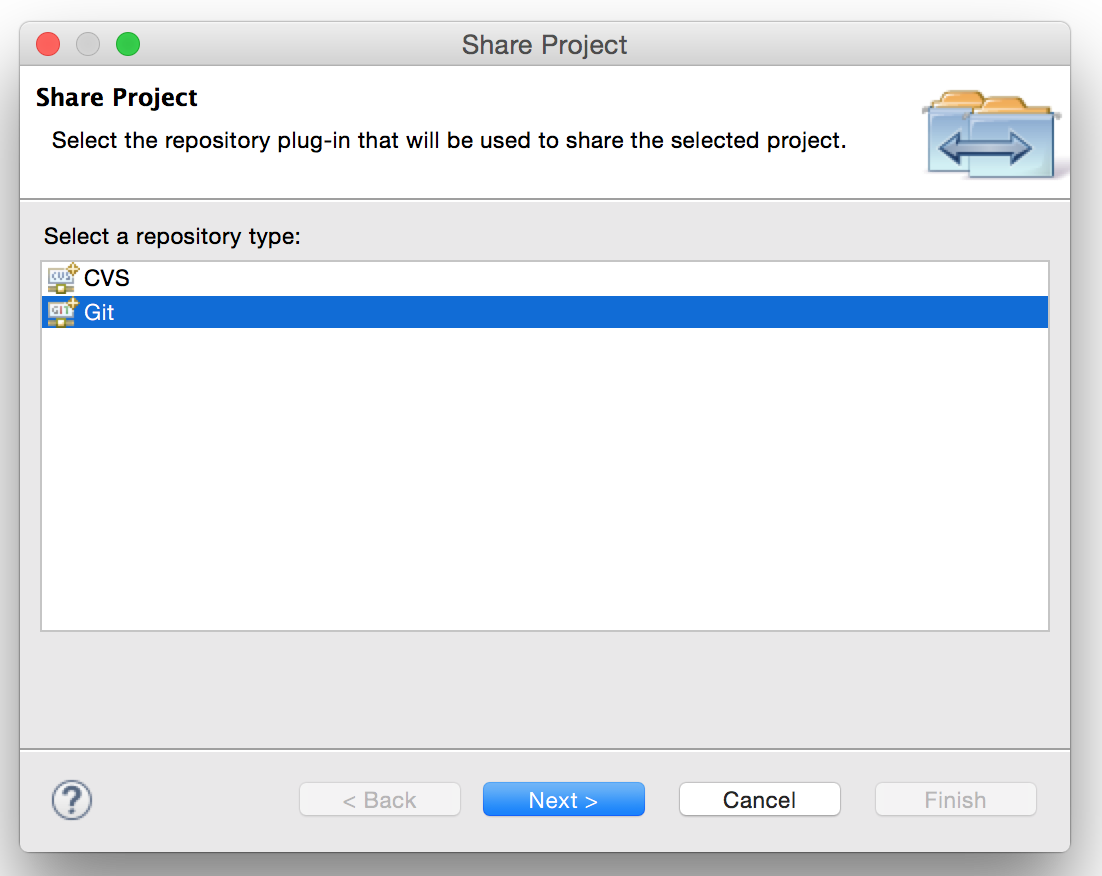
\includegraphics[scale=0.5]{figures/s4.png}
\end{center}

\begin{center}
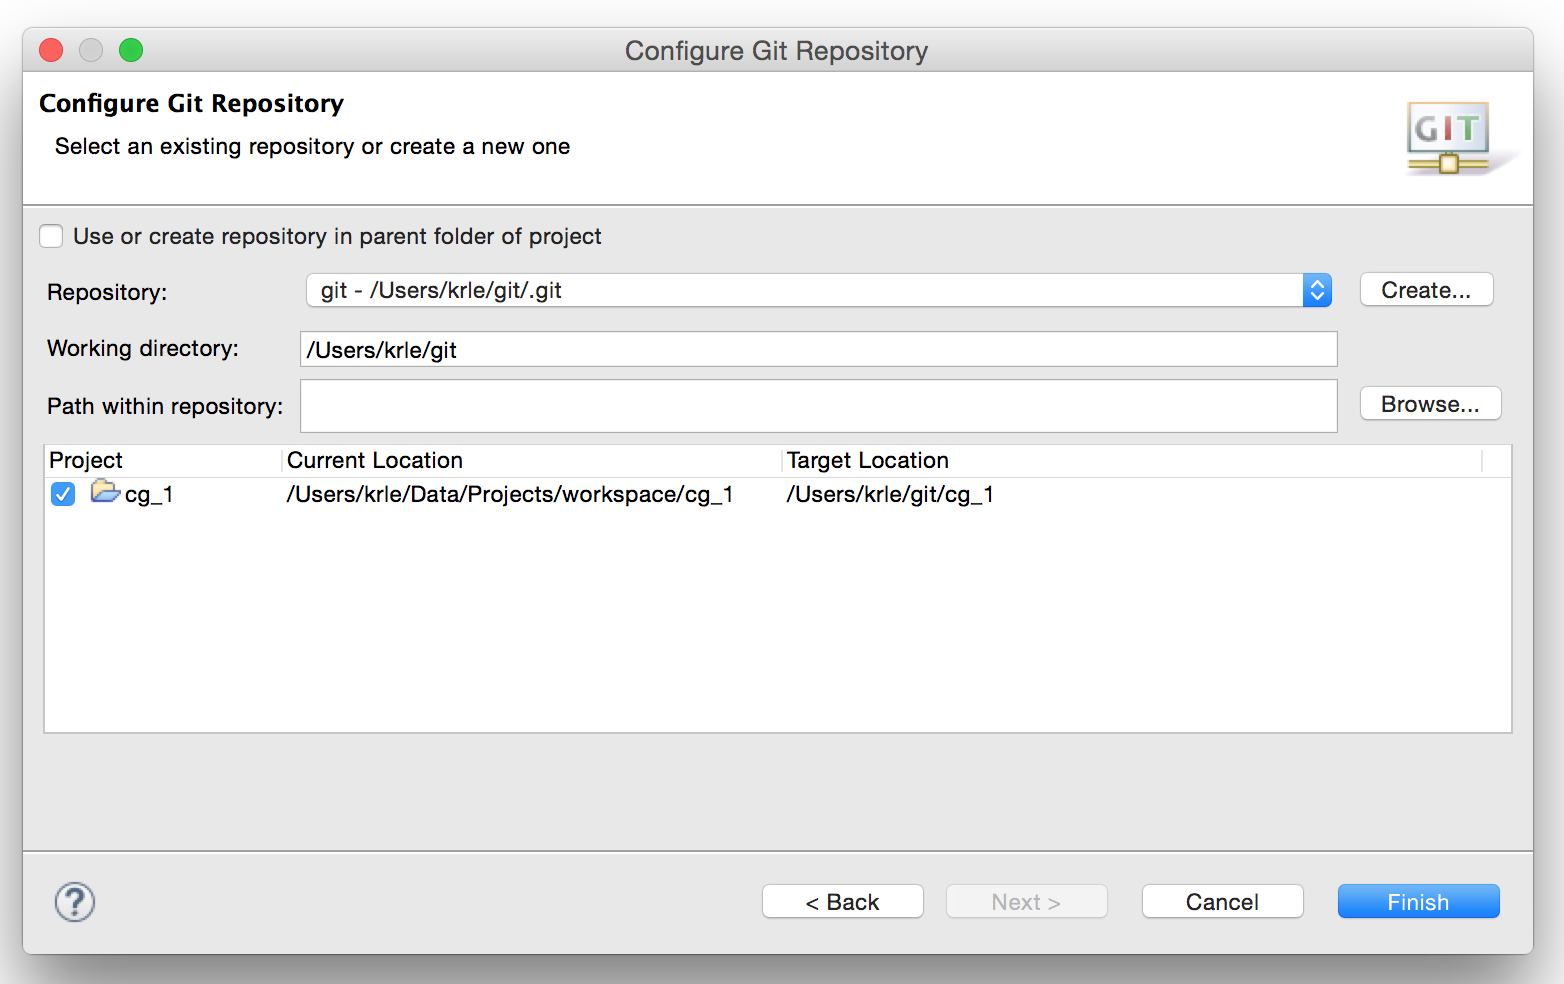
\includegraphics[scale=0.5]{figures/s5.png}
\end{center}

It is recommended to separate your Git repository from any additional
meta-data which Eclipse might create, it is recommended to place your
Git repositories outside the Eclipse workspace. Eclipse follows this
recommendation and the EGit plug-in proposes a directory outside your
workspace. Placing Git repositories directly in the workspace may
cause performance issues since the Git support in Eclipse then may
need to scan a large number of files reachable under the workspace. 

Once you click ok all the project contents in your workspace are going
to be copied to the working directory you specified.

\begin{center}
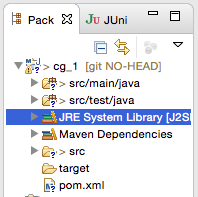
\includegraphics[scale=0.6]{figures/s6.png}
\end{center}

You should see the project structure like in the above figure.
The ``> '' sign means that folder or file has uncommitted changes.


\item Edit the .gitignore file in your working directory

Git can be configured to ignore certain files and directories for
repository operations. This is configured via one or several
.gitignore files. Typically, this file is located at the root of your
Git repository but it can also be located in sub-directories. In the
second case the defined rules are only valid for the sub-directory and
below. 

Here is a typical .gitignore file

\begin{lstlisting}
# ignore all bin directories
# matches "bin" in any subfolder
bin/

# ignore all target directories
target/

# ignore all files ending with ~
*~ 

# ignore metadata directories
.metadata

# ignore DS_Store and files starting with ._ (for Mac)  
.DS_Store
._*
\end{lstlisting}

The rule is NEVER to commit files that can be derived
automatically. In practice for a maven project this usually means only
pom.xml file and src/ folder should be under version control.

NOTE: You can also configure Eclipse to automatically ignore derived
resources, e.g. class files via the 
Window $\rightarrow$ Preferences
$\rightarrow$ Team $\rightarrow$ Git $\rightarrow$ Projects
$\rightarrow$ Automatically ignore derived resources  (for Windows or Linux)
or\\
Eclipse $\rightarrow$ Preferences
$\rightarrow$ Team $\rightarrow$ Git $\rightarrow$ Projects
$\rightarrow$ Automatically ignore derived resources

\item Stage your changes

Eclipse gives you several options to stage and commit your
changes. The Git Staging view provides a convenient compact overview
on all changes you have done since checking out a branch.



Click on the Git repository view in the upper right corner (usually
next the Java view which is currently selected).

Select your newly created repository in the left.

Than in the bottom tabs choose git staging.

\begin{center}
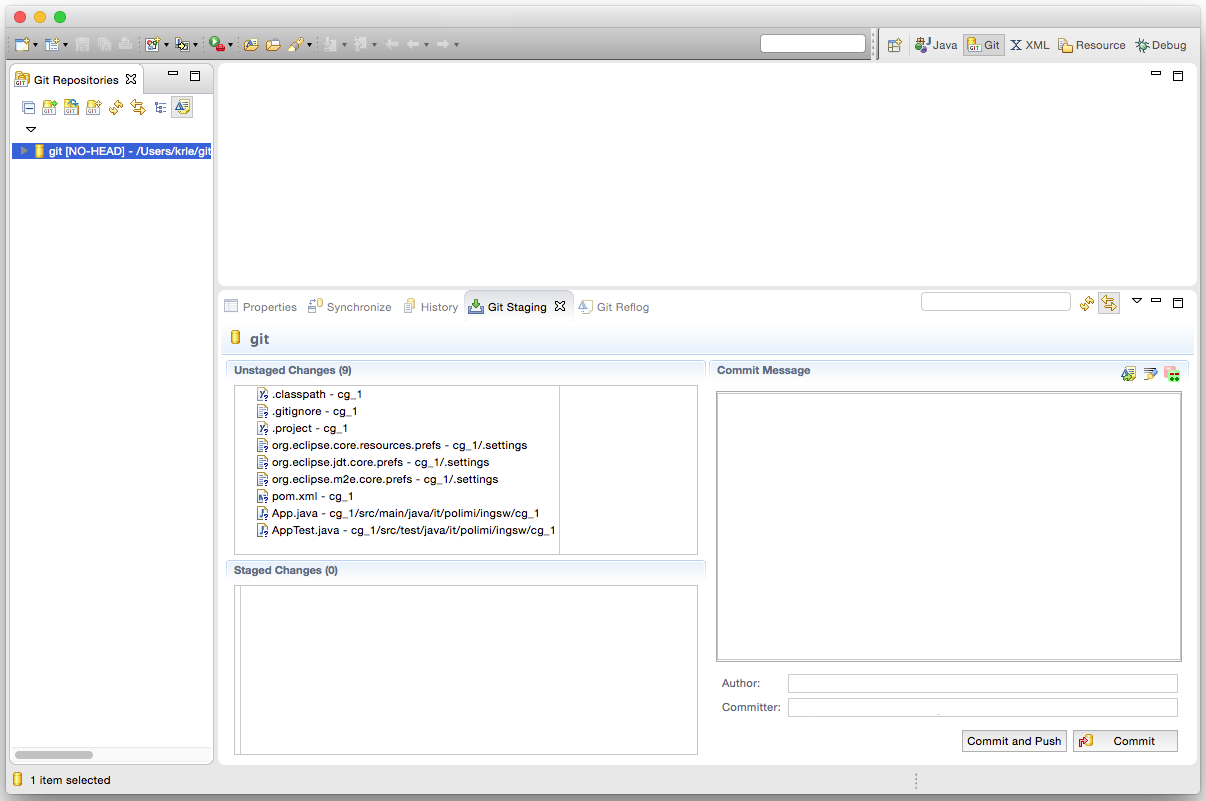
\includegraphics[scale=0.33]{figures/s7.png}
\end{center}

Select .gitignore, pom.xml, App.java and AppTest.java files and
transfer them into the lower part for staging.

\begin{center}
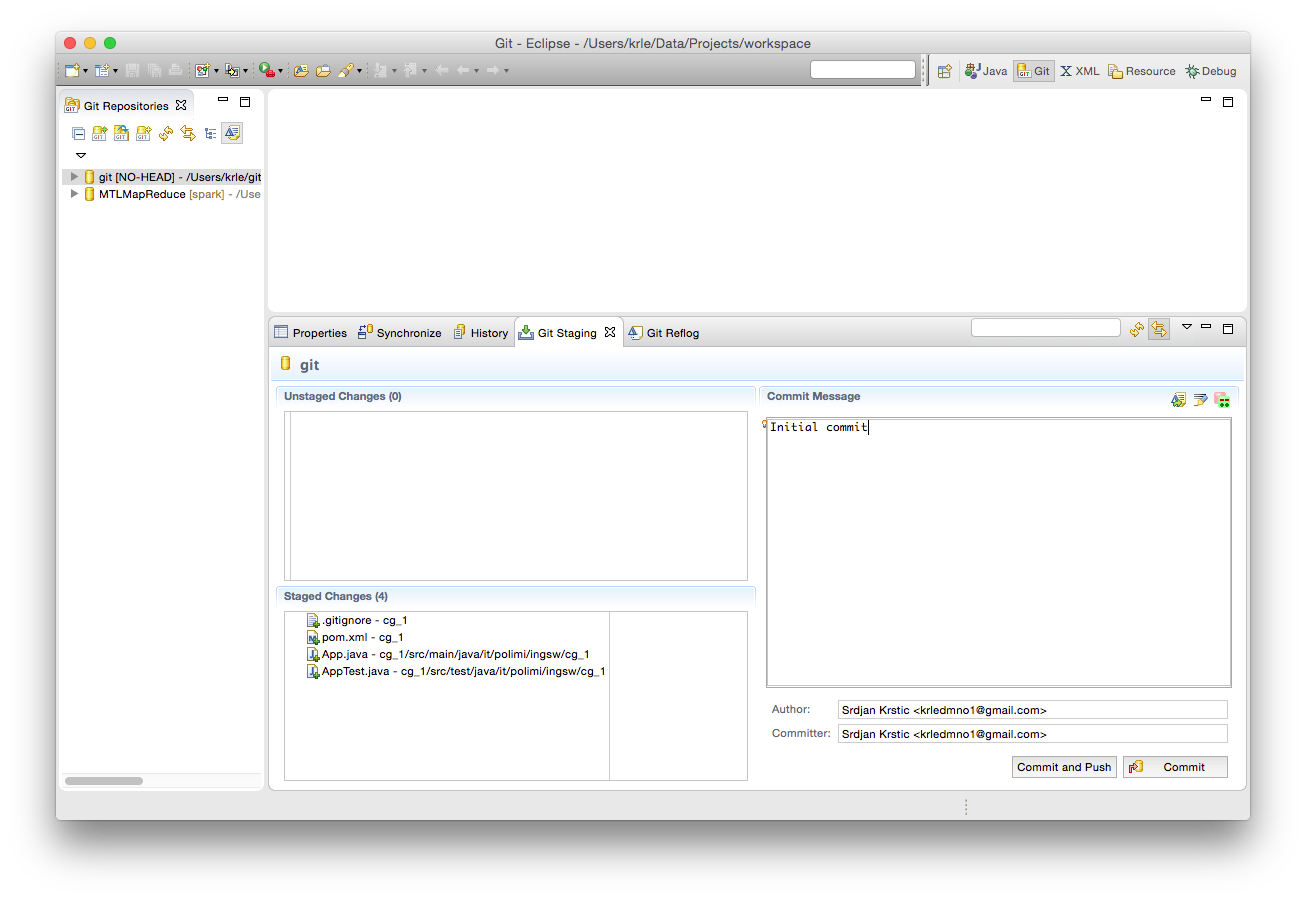
\includegraphics[scale=0.33]{figures/s8.png}
\end{center}

\item Commit

Write a commit message and press commit.
Once you return to Java view you can the the following project
structure. Notice that the symbols have changed to reflect that the
current version is saved in the repository.

\begin{center}
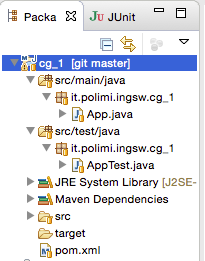
\includegraphics[scale=0.6]{figures/s9.png}
\end{center}

NOTE: A quicker way to commit is to right click on the project, choose 
Team $\rightarrow$ Commit... and then choose the files to stage.

\item Connect and push to the remote repository

Right click on the project and choose Team $\rightarrow$ Push...
Write the correct uri path (that we are going to provide to you in the
lab) like in the example figure: 

\begin{center}
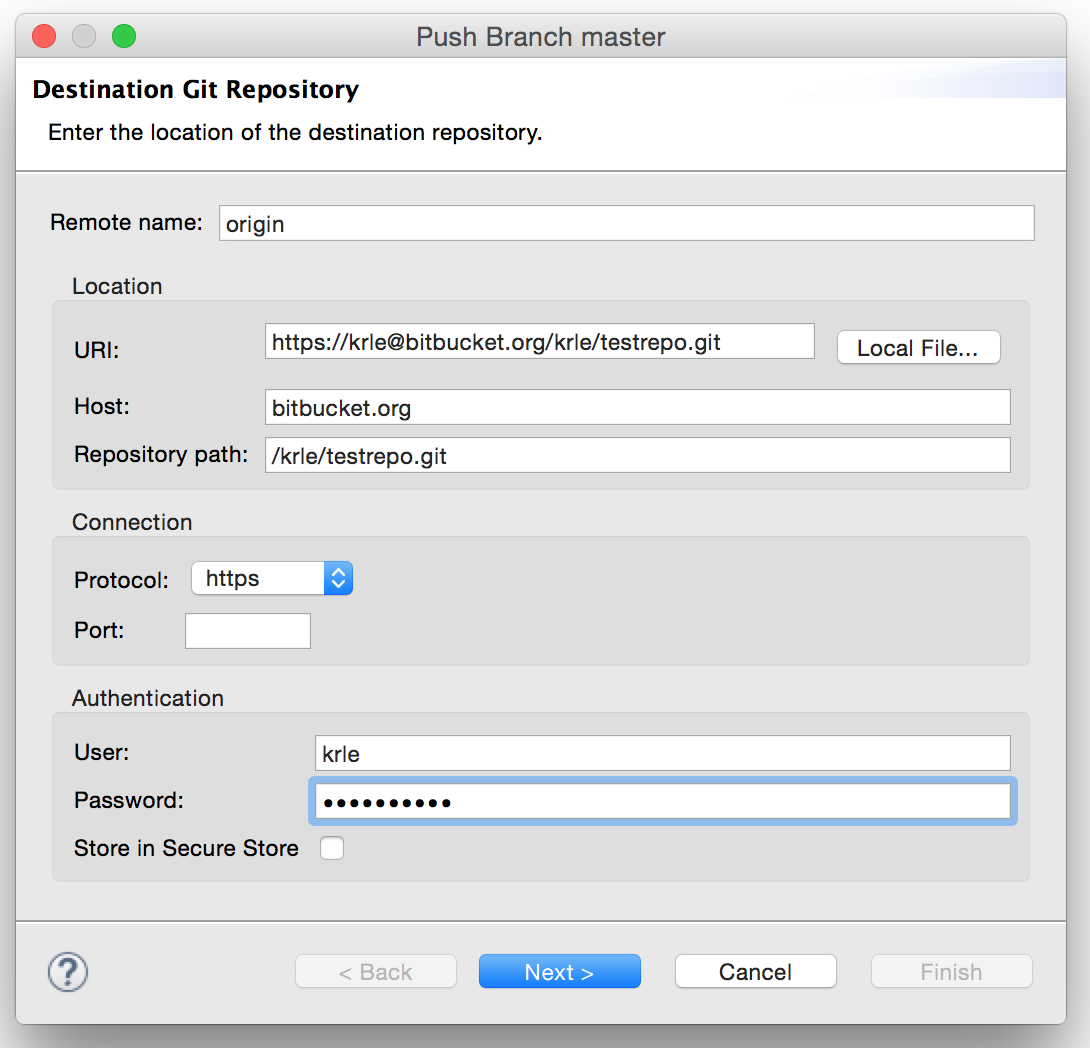
\includegraphics[scale=0.35]{figures/s10.png}
\end{center}

Press next and then finish.
The remote repository should now show all the commits.

\end{enumerate}

\subsection{Clone existing project}

\subsection{Collaborate}


\section{Git workflows}

\end{document}

